\documentclass[italian]{beamer}
\usetheme{CambridgeUS}
\setbeamertemplate{navigation symbols}{}
\setbeamertemplate{itemize item}[circle]
\setbeamertemplate{itemize subitem}[square]
\definecolor{cambridgeusred}{RGB}{163,0,0}
\setbeamercolor{structure}{fg=cambridgeusred}

\usepackage[italian]{babel}
\usepackage{amsfonts}
\usepackage{graphicx}
\graphicspath{{./images/}}
\usepackage{circuitikz}
\usepackage{hyperref}

\title{Misure su un circuito crossover}
\author{Enrico Barbuio}
\institute[]{Laboratorio di Elettromagnetismo e Ottica \\ Corso di laurea triennale in Fisica}
\date{9 luglio 2025}

\begin{document}

{
\setbeamertemplate{footline}{} %empty footline for title
\maketitle
}
\setbeamertemplate{footline}[cambridgeus]

\begin{frame}{Obiettivo}
    \begin{itemize}
        \item Progettazione di un circuito crossover a tre vie
        \item Analisi del comportamento in regime sinusoidale:
              \begin{itemize}
                  \item Studio qualitativo e quantitativo della risposta in frequenza di ampiezza e fase per ciascun canale del filtro.
                  \item Misura di frequenza di crossover, frequenza di risonanza e fattore di qualità
                  \item Confronto con valori e comportamento atteso
              \end{itemize}
    \end{itemize}
\end{frame}

\begin{frame}{Circuito e scelta dei componenti}
    \begin{columns}
        \begin{column}{0.65\textwidth}
            \centering
            \begin{circuitikz}[scale=0.6, transform shape]
                % generatore
                \draw (9.5,0) --
                (0,0) --
                (0,1.5) to[sinusoidal voltage source, label=$v_0$]
                (0,3) to[R, l=$R_g$, color=cambridgeusred, bipoles/resistor/height=0.15, bipoles/resistor/width=0.5]
                (0,4) --
                (0,5.5) --
                (9.5,5.5);

                \draw(0,4.5) to[short, -o]
                (-0.6,4.5) node[left]{$v_g$};
                \draw (0,1) -- (-0.6,1) node[ground]{};

                % woofer
                \draw (3,5.5) --
                (3,5) to[L=$L_w$]
                (3,3.5) to[R, l=$R_{Lw}$, color=cambridgeusred, bipoles/resistor/height=0.15, bipoles/resistor/width=0.5]
                (3,2.5) --
                (3,2) to[R=$R_w$] (3,0);
                \draw (3,2) to [short, -o] (3.6, 2) node[right]{$v_w$};

                % mid
                \draw (6, 5.5) -- (6, 5.25);

                \draw (6, 5.25) -- (6.5,5.25) to [C=$C_m$] (6.5,4.25) -- (6, 4.25);

                \draw (6, 5.25) --
                (5.5, 5.25) to [R, l_=$R_{Cm}$, color=cambridgeusred, bipoles/resistor/height=0.15, bipoles/resistor/width=0.5]
                (5.5, 4.25) --
                (6, 4.25);

                \draw(6,4.25) to [L=$L_m$]
                (6,3) to [R, l=$R_{Lm}$, color=cambridgeusred, bipoles/resistor/height=0.15, bipoles/resistor/width=0.5]
                (6,2) --
                (6,2) to[R=$R_m$] (6,0);

                \draw (6,2) to [short, -o] (6.6, 2) node[right]{$v_m$};

                %tweeter
                \draw (9.5,5.5) --
                (9.5, 4.25);

                \draw (9.5, 4.25) -- (10,4.25) to [C=$C_m$] (10,3.25) -- (9.5, 3.25);

                \draw (9.5, 4.25) --
                (9, 4.25) to [R, l_=$R_{Cm}$, color=cambridgeusred, bipoles/resistor/height=0.15, bipoles/resistor/width=0.5]
                (9, 3.25) --
                (9.5, 3.25);

                \draw(9.5, 3.25) --
                (9.5,2) to[R=$R_t$] (9.5,0);

                \draw (9.5,2) to
                [short, -o] (10.1, 2) node[right]{$v_t$};
            \end{circuitikz}
        \end{column}
        \begin{column}{0.2\textwidth}
            \begin{alignat*}{2}
                 & R &  & = 3\text{k}3 \text{ \Omega} \\
                 & L &  & = 47 \text{ mH}             \\
                 & C &  & = 4.7 \text{ nF}
            \end{alignat*}
        \end{column}
    \end{columns}

    \bigskip

    I componenti sono stati scelti secondo questi criteri:
    \begin{itemize}
        \item Sfruttare le capacità di acquisizione di Elvis II ($1$ MS/s)\\
              \Rightarrow\ Frequenza di Crossover e Risonanza $f_c \approx f_r \approx 10$ kHz
        \item Minimizzare la caduta di potenziale sulla resistenza interna al generatore
              \Rightarrow\ resistenze di carico grandi
    \end{itemize}
\end{frame}

\begin{frame}{Acquisizione dati}
    Componenti misurati con multimetro digitale di Elvis II.

    \bigskip
    Interesse principale: dominio delle frequenze:
    \begin{itemize}
        \item Acquisizione di tensioni su due canali alla volta. Sweep ripetuti e successiva sovrapposizione
        \item Campionamento a $500$ kHz per canale con buffer di $2000$ sample e trigger analogico
        \item Misure di tensioni in modalià RSE
    \end{itemize}

\end{frame}
\begin{frame}{Elaborazione dati}
    Da ciascun campione di onda sinusoidale sono stati estratti e graficati ampiezza e fase in funzione della frequenza.

    \begin{itemize}
        \item Incertezza sulla fase: deviazione standard su misure ripetute \rightarrow\ $\sigma_\phi = 0.003^\circ$
        \item Incertezza statistica sull'ampiezza inferiore alla risoluzione strumentale
              \rightarrow\ risoluzione della scheda: $\Delta V = 1.9$ mV
    \end{itemize}

    Le fasi sono calcolate come differenza di fase tra \texttt{A1} e \texttt{A0}.
    Per correggere la deriva dovuta al multiplexing: fit lineare sul generatore connesso ad \texttt{A1}.
\end{frame}

\begin{frame}{Grafico ampiezza - frequenza}
    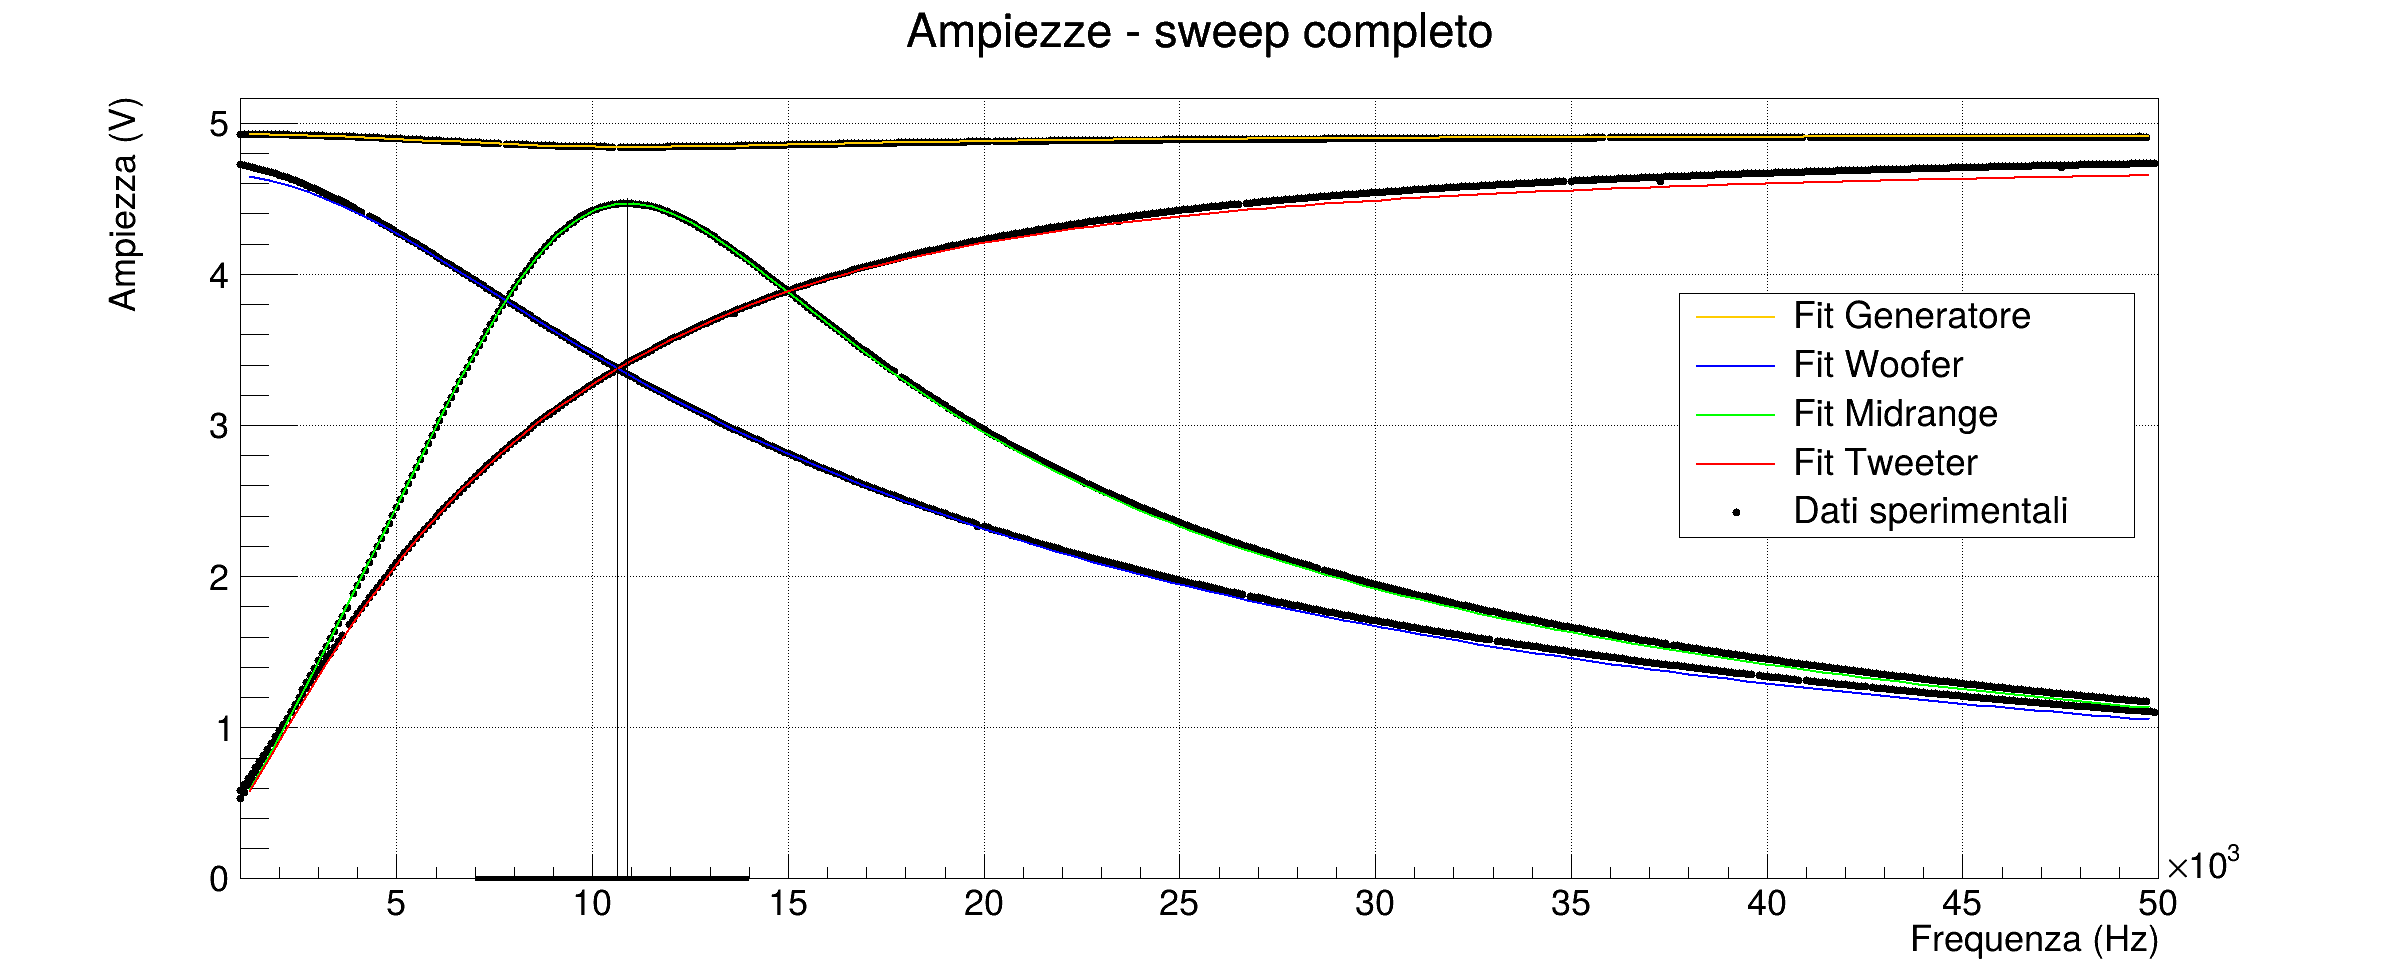
\includegraphics[width=\textwidth]{fig_amp.png}
    Fit convergente solo su dominio ristretto ($7$ - $14$ kHz).\\
    Andamento coerente con quello atteso:
    \begin{itemize}
        \item[\checkmark] Woofer \rightarrow\ filtro passa-basso
        \item[\checkmark] Midrange \rightarrow\ filtro passa-banda
        \item[\checkmark] Tweeter \rightarrow\ filtro passa-alto
    \end{itemize}
\end{frame}

\begin{frame}{Grafico fase - frequenza}
    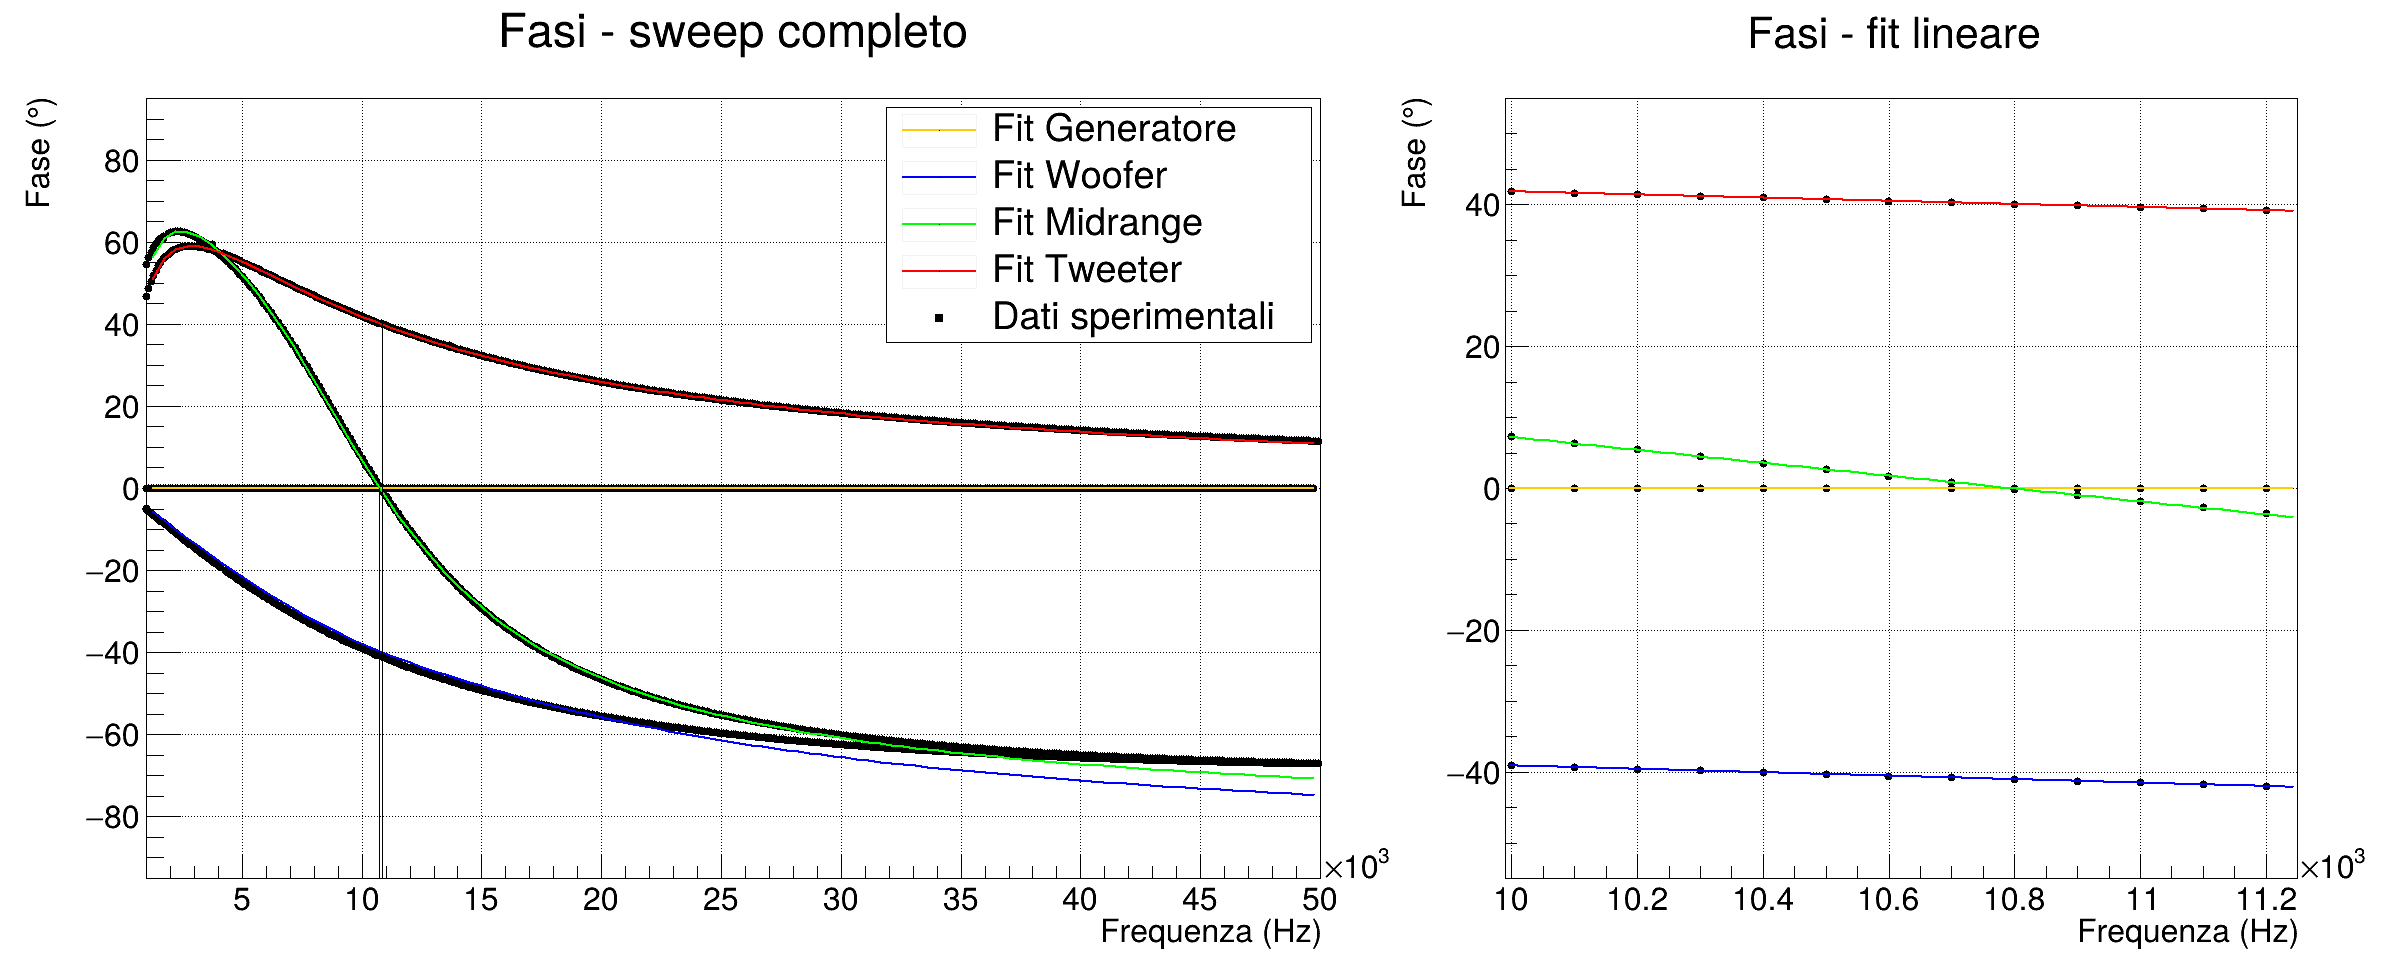
\includegraphics[width=\textwidth]{fig_fase.png}
    Difficoltà nell'ottenere un fit convergente, grande instabilità nei parametri e dipendenza dal range di fit.
    Per ottenere misure significative: fit lineare su range ristretto.

    Sotto i $\sim 5$ kHz: abbassamento fase su midrange e tweeter, modellato dalla resistenza in parallelo dei condensatori.
\end{frame}

\begin{frame}{Misure attese e misure sperimentali}
    Misure attese: leggi di Kirchoff e legge di Ohm generalizzata.\\
    Misure sperimentali: media pesata delle misure ricavate da ampiezze e fasi.

    \begin{itemize}
        \item Frequenza di crossover:
              \begin{equation*}
                  f_{c}^{sper} = (10.61 \pm 0.03) \text{ kHz} \hspace{2cm} f_{c}^{teo} = (10.50
                  \pm 0.12) \text{ kHz}
              \end{equation*}
        \item Frequenza di risonanza:
              \begin{equation*}
                  f_{r}^{sper} = (10.80 \pm 0.09) \text{ kHz} \hspace{2cm} f_{r}^{teo} = (10.65
                  \pm 0.10) \text{ kHz}
              \end{equation*}
        \item Fattore di qualità del passa-banda del midrange:
              \begin{equation*}
                  Q^{sper} = 0.88 \pm 0.12  \hspace{2cm}  Q^{teo} = 0.954 \pm 0.010
              \end{equation*}
    \end{itemize}
    Intervalli di incertezza dati da un fattore di copertura $3$
\end{frame}

\begin{frame}{Conclusioni}
    \begin{itemize}
        \item Le misure sperimentali di $f_c$, $f_r$, $Q$ risultano compatibili con i valori attesi.

        \item Pur tenendo conto di effetti non ideali il modello non è perfetto.
              \begin{itemize}
                  \item Per le ampiezze il modello è accurato ma si può dire propriamente compatibile solo su range ristretto
                  \item Per le fasi ci sono importanti effetti sistematici sulle alte frequenze
              \end{itemize}

        \item L'abbassamento delle fasi a basse frequenze su tweeter e woofer può essere dovuto a correnti
              di dispersione nei condensatori, modellate come resistenze in parallelo.
              Dal fit $R_{Cm} \approx R_{Ct} \approx 40$ k\Omega, ma misurando con il multimetro risulta un circuito aperto.
    \end{itemize}
\end{frame}

\begin{frame}[b]{Fine - Materiale aggiuntivo}
    \Large\centerline{Fine della presentazione.}

    \vspace{8em}

    \small
    La relazione completa, i dati e le macro per l'analisi sono reperibili al seguente link:
    \url{github.com/enro284/lab2_circuiti}
\end{frame}
\end{document}